\subsubsectionwithauthor[author={Mika Landeck},email={mika.landeck@fau.de}]{Aufgabe 1: Reguläre Sprachen}

\paragraph{(a)}m
	$L=(a|b|c)^*b(a|c)(c|ba)^*$		
	
\paragraph{(b)}m
	\underline{Schritt 1:} Umwandlung des NEA zum DEA mittels Potenzmengenkonstruktion:
	
	\begin{tabular}{c|c|c|c|c|l}
		\textbf{Zustand} & \textbf{Eingabe a} & \textbf{Eingabe b} & \textbf{Eingabe c} & \textbf{Final} & \textbf{Anmerkung} \\
		\hline
		q                & q                  & qr                 & q                  &                   & Neuer Zustand qr \\
		\hline
		qr               & qs                 & q                  & qs                 &                   & Neuer Zustand qs \\
		\hline
		qs               & q                  & qt                 & qs                 &  $\checkmark$                 & Neuer Zustand qt\\
		\hline
		qt               & qs                 & q                  & q                 &                   & \\
		\hline
	\end{tabular}
	
	Der Tabelle können aus der ersten Spalte die für den DEA benötigten Zustände entnommen werden. Zudem werden die Übergänge nach Eingabe von $a$, $b$ oder $c$ aufgeführt und die Endzustände gekennzeichnet.
	
	\underline{Schritt 2:} Der gesuchte DEA soll aber nicht $L$, sondern das Komplement von $L$ erkennen. Um das zu erreichen, werden Endzustände und Nicht-Endzustände vertauscht. Hier die graphische Darstellung des gesuchten DEA, der $\overline{L}$ akzeptiert:
	
	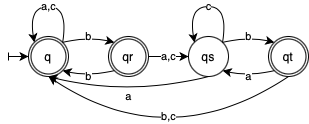
\includegraphics[scale=0.8]{Komplement-DEA}
		
\paragraph{(c)}m
	\underline{Schritt 1:} Angabe einer Zeugentabelle zur Überprüfung der Erreichbarkeit:

	\begin{tabular}{l|ccccccc}
		\textbf{Zustand} & q & r  & s          & t & x  & y & z \\
		\hline
		\textbf{Zeuge}   & 1 & 11 & $\epsilon$ & - & 01 & 0 & 00 \\
	\end{tabular} 
	
	Der Zustand t ist also nicht erreichbar und entfällt im minimierten Automaten.
	
	\underline{Schritt 2:} Identifizieren nicht äquivalenter Zustände über Tabelle mit Zustandspaaren:
	
	\includegraphics[scale=0.6]{Tabellenfüllverfahren.png}

	\textbf{Tabellenfüllverfahren} \\
	Zunächst werden alle Zustandspaare, die aus einem Endzustand und einem Nicht-Endzustand bestehen, mit X0 markiert. Weitere Kreuze in der Tabelle findet man mittels folgender Übergangstabelle von Zustandspaaren:

	\begin{tabular}{c|c|c|l}
		\textbf{Zustandspaar} & \textbf{0} & \textbf{1} & \textbf{Erläuterung} \\
		\hline
		(s,r)                 & (y,q)      & (q,x)      & Eingabe 0 führt mit (y,q) zu X0. Ergänze X1. \\
		\hline
		(x,r)                 & (r,q)      & (z,x)      & Eingabe 0 führt mit (r,q) zu X0. Ergänze X2. \\
		\hline
		(x,s)                 & (r,y)      & (z,q)      & Eingabe 1 führt mit (z,q) zu X0. Ergänze X3. \\
		\hline
		(y,s)                 & (z,y)      & (x,q)      & Eingabe 1 führt mit (z,q) zu X0. Ergänze X4. \\
		\hline
		(y,x)                 & (z,r)      & (z,x)      & Eingabe 1 führt mit (z,x) zu X0. Ergänze X5. \\
		\hline
		(z,q)                 & (x,x)      & (y,r)      & z und q sind äquivalent. \\
		\hline 		
		(y,r)                 & (z,q)      & (x,x)      & y und r sind äquivalent. \\
	\end{tabular} 
	
	Die Zustände $z$ und $q$ sowie $y$ und $r$ sind äquivalent, da auch bei wiederholter Überprüfung keine Übergänge gefunden werden, die zu einem Kreuz führen. Damit ergeben sich für den minimierten Automaten folgende Zustände, die den Äquivalenzklassen der Zustände von $A$ entsprechen: $[z,q],[y,r],[s],[x]$
	
	Der minimierte Automat A' lautet also: \\
	$A' = (\{[q,z],[y,r],[s],[x]\},\{0,1\},\delta',[s],\{[q,z]\})$ mit

	\begin{tabular}{c|c|c}
		$\delta'$ & 0 & 1 \\
		\hline
		[s]       & [y,r]      & [q,z] 	\\
		\hline
		[x]       & [y,r]      & [q,z]	\\
		\hline
		[y,r]     & [q,z]      & [x]	\\
		\hline
		[q,z]     & [x]        & [y,r]	\\
	\end{tabular}


\newpage